\section{Creación de un Cubo}  

En el Solution Explorer nos ubicamos en Cubes y click derecho, seleccionando la opción de New Cube …
	\begin{center}
	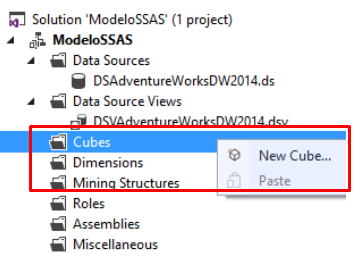
\includegraphics[width=8cm]{images/task3/img15}
	\end{center}	
Se nos abrirá una ventana de resumen. Click en Next:
	\begin{center}
	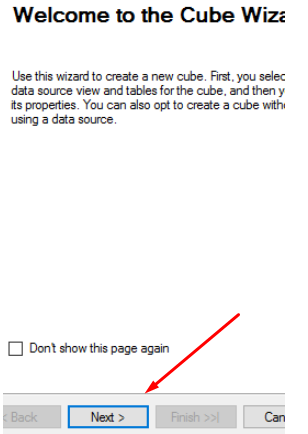
\includegraphics[width=8cm]{images/task3/img16}
	\end{center}	
Para la creación de un cubo tenemos varias opciones.
Use existing tables: Utilizar tablas del Data Source View.
Create an empty cube: Crear un cubo vacío.
Generate tables in the data source: Nos da la opción de crear tablas a partir de templates.
En este caso utilizaremos las tablas seleccionadas en el Data Source View creada en la sección 2:
	\begin{center}
	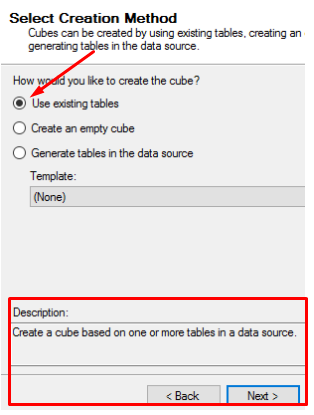
\includegraphics[width=8cm]{images/task3/img17}
	\end{center}	
Click en Next.
Aquí seleccionaremos la FactTable (Tablas de Hechos) , en este caso ubicamos FactInternetSales:
	\begin{center}
	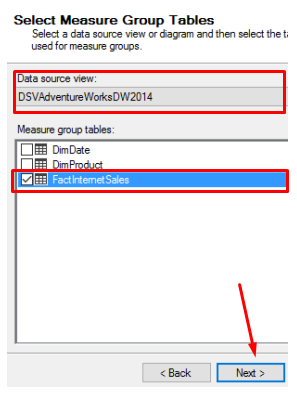
\includegraphics[width=8cm]{images/task3/img18}
	\end{center}	
Click en Next.
Automáticamente el Data Tools identificará todos los campos numéricos y los marcará como candidatos a
ser medidas. Podemos observar que inclusive marca los campos utilizados como Foregin Keys. En este
caso, seleccionamos solo Order Quantity y Sales Amount:
	\begin{center}
	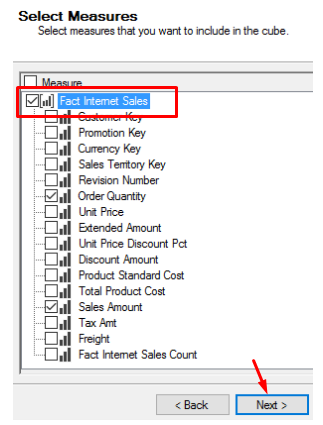
\includegraphics[width=8cm]{images/task3/img19}
	\end{center}	
Click en Next.
Aquí seleccionamos las dimensiones por las cuales será analizada la data. Inclusive el Data Tools te indica
que podría tomar la misma FactTable como Dimensión. Seleccionamos Dim Date y Dim Product:
	\begin{center}
	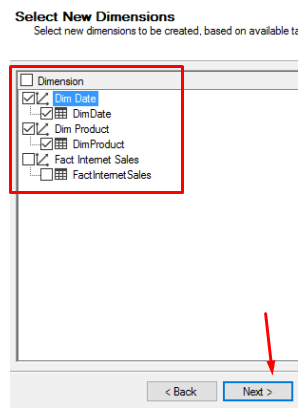
\includegraphics[width=8cm]{images/task3/img20}
	\end{center}	
Click en Next.
Colocamos un nombre el cubo:

	\begin{center}
	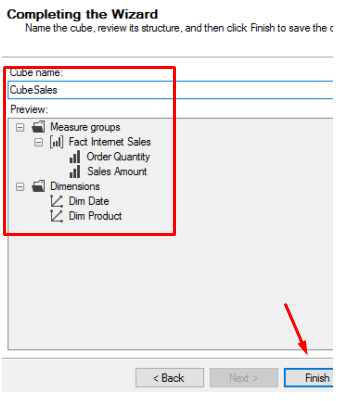
\includegraphics[width=8cm]{images/task3/img21}
	\end{center}	

Click en Finish